\documentclass{article}
\usepackage{graphicx} % Required for inserting images
\usepackage{geometry}
\usepackage{circuitikz}
\usepackage{siunitx}
\usepackage{CJKutf8}
\usepackage{amsmath}
\usepackage{amssymb}
\usepackage{caption}
\usepackage{float}
\usepackage{subcaption}
\geometry{top=5mm, left=30mm, a4paper}

\title{CMOS Operational Amplifier Prelab}
\author{梁程捷 (B11901136), 吳奕娃 (B11901080)}
\date{}


\begin{document}
\begin{CJK*}{UTF8}{bkai}

\maketitle

\section*{CMOS Operational Amplifier Small Signal Analysis}
Use three CD4007 ICs to construct the circuit in Figure (a) or Figure (b), and follow the steps below: \\
1. Record the input($V_i$) and output($V_o$) waveform in Y-t mode for f=1\unit{\kilo\hertz}. \\
2. Plot the magnitude bode diagram of $V_o$/$V_i$ for f=500\unit{\kilo\hertz} to 1\unit{\mega\hertz}. \\
3. Indicate the 3-dB frequency and the bandwidth. \\
note: For Each CD4007 IC, supply voltage VSS = –8V in pin 7 and VDD = +8V in pin 14. \\

\begin{figure}[h]
    \begin{center}
    
        \begin{subfigure}[b]{0.45\textwidth}
            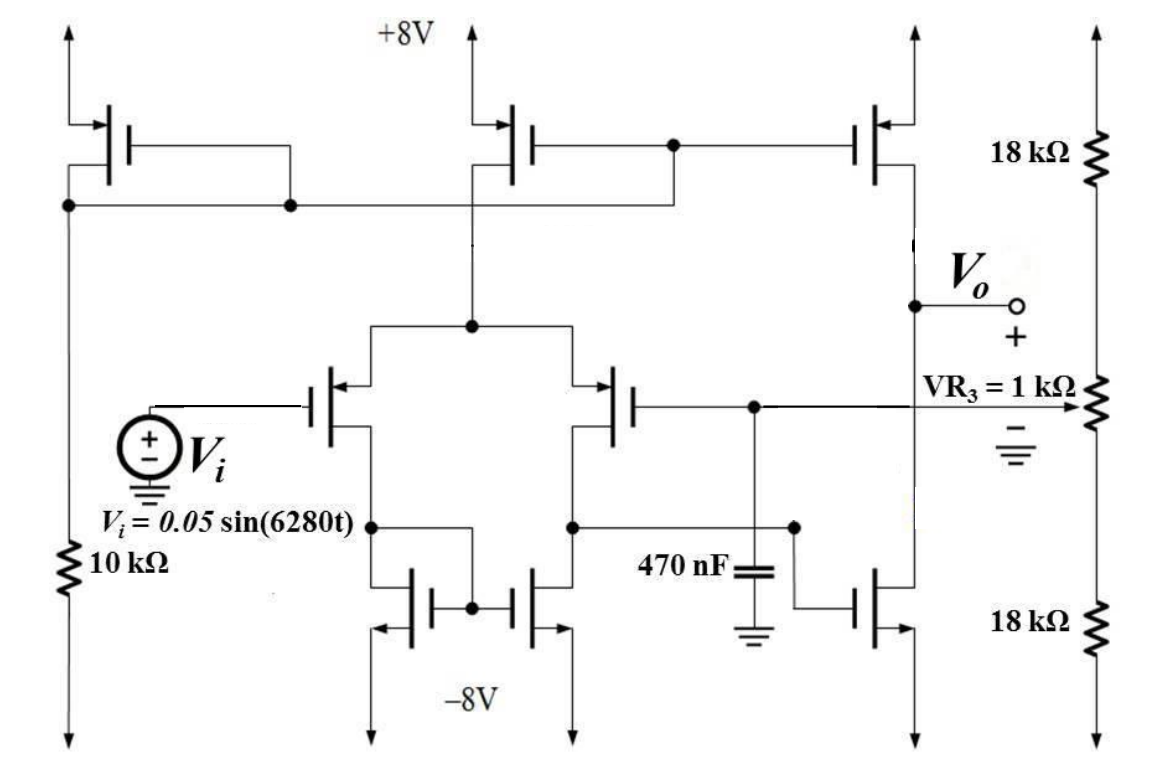
\includegraphics[width=\textwidth]{CMOS_simple.png}
            \caption*{Figure (a)}
        \end{subfigure}
        ~
        \begin{subfigure}[b]{0.45\textwidth}
            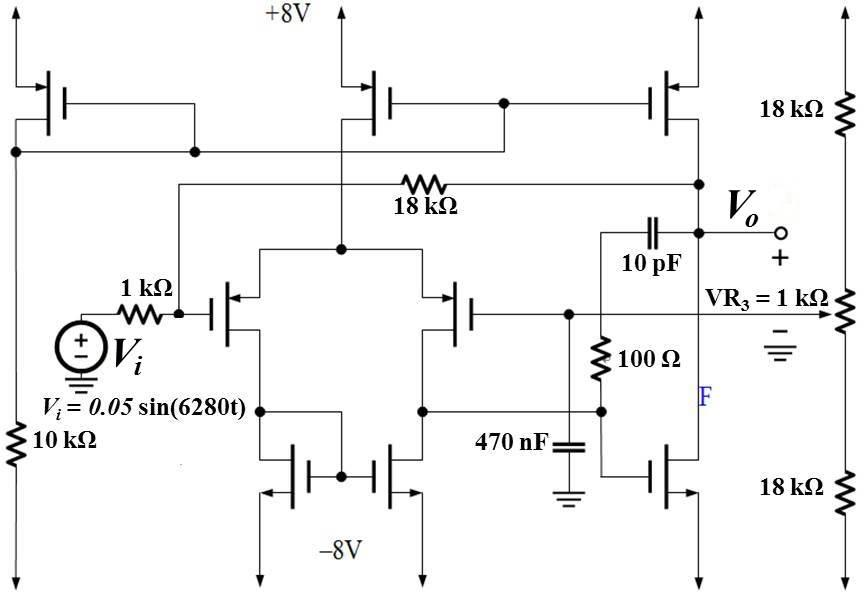
\includegraphics[width=\textwidth]{CMOS_complicated.png}
            \caption*{Figure (b)}
        \end{subfigure}
    \end{center}
\end{figure}

% \textbf{FET model: BS170} \\
% \textbf{Voltage source:} $V_{DD} = +15$ \unit{\volt}; $v_{sig} = 0.2 \sin(2 \pi f t)$, $f = 200$ \unit{\hertz} $\sim$ 500 \unit{\kilo\hertz}\\
% \textbf{Resistors: }$R_{G1} = R_{G2} = 1$ \unit{\mega\ohm}; $R_D = R_S = R_L = 10$ \unit{\kilo\ohm}; $R_{sig} = 100$ \unit{\kilo\ohm}\\
% \textbf{Capacitors: }$C_{C2} = C_S = 0.1$ \unit{\micro\farad} (104); $C_{C1} = 0.01$ \unit{\micro\farad} (103)\\

\begin{figure}[h]
    \begin{center}
        \begin{subfigure}[b]{0.45\textwidth}
            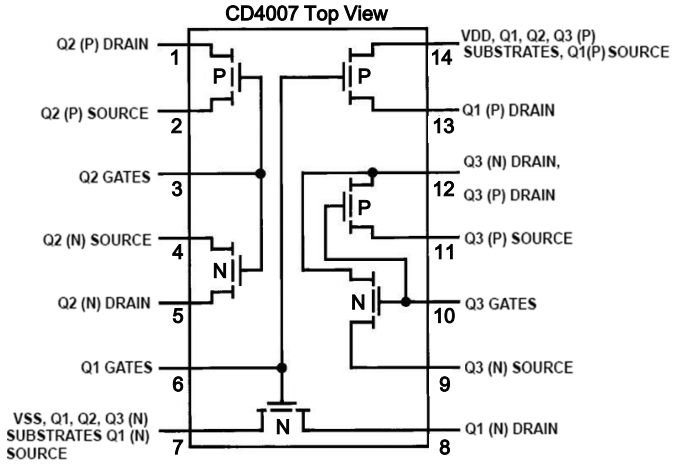
\includegraphics[width=\textwidth]{CD4007_IC.png}
            \caption*{Figure (c): the CD4007 IC}
        \end{subfigure}
    \end{center}
\end{figure}
    
\end{CJK*}
\end{document}